% =========================================================
\section{TEF-RAG 方法}
\label{sec:method}
% =========================================================

图~\ref{fig:tef_overview} 展示了 TEF-RAG 的整体流程。该方法由四个相互连接的阶段组成：合法候选检索、学习式证据对提议、查询条件化关系图构建以及非线性集合排序。前两个阶段用于控制候选规模，关系图用于表示证据记录之间的过程结构，最终排序器则直接比较不同候选证据集合的整体效用。

\begin{figure*}[t]
    \centering
    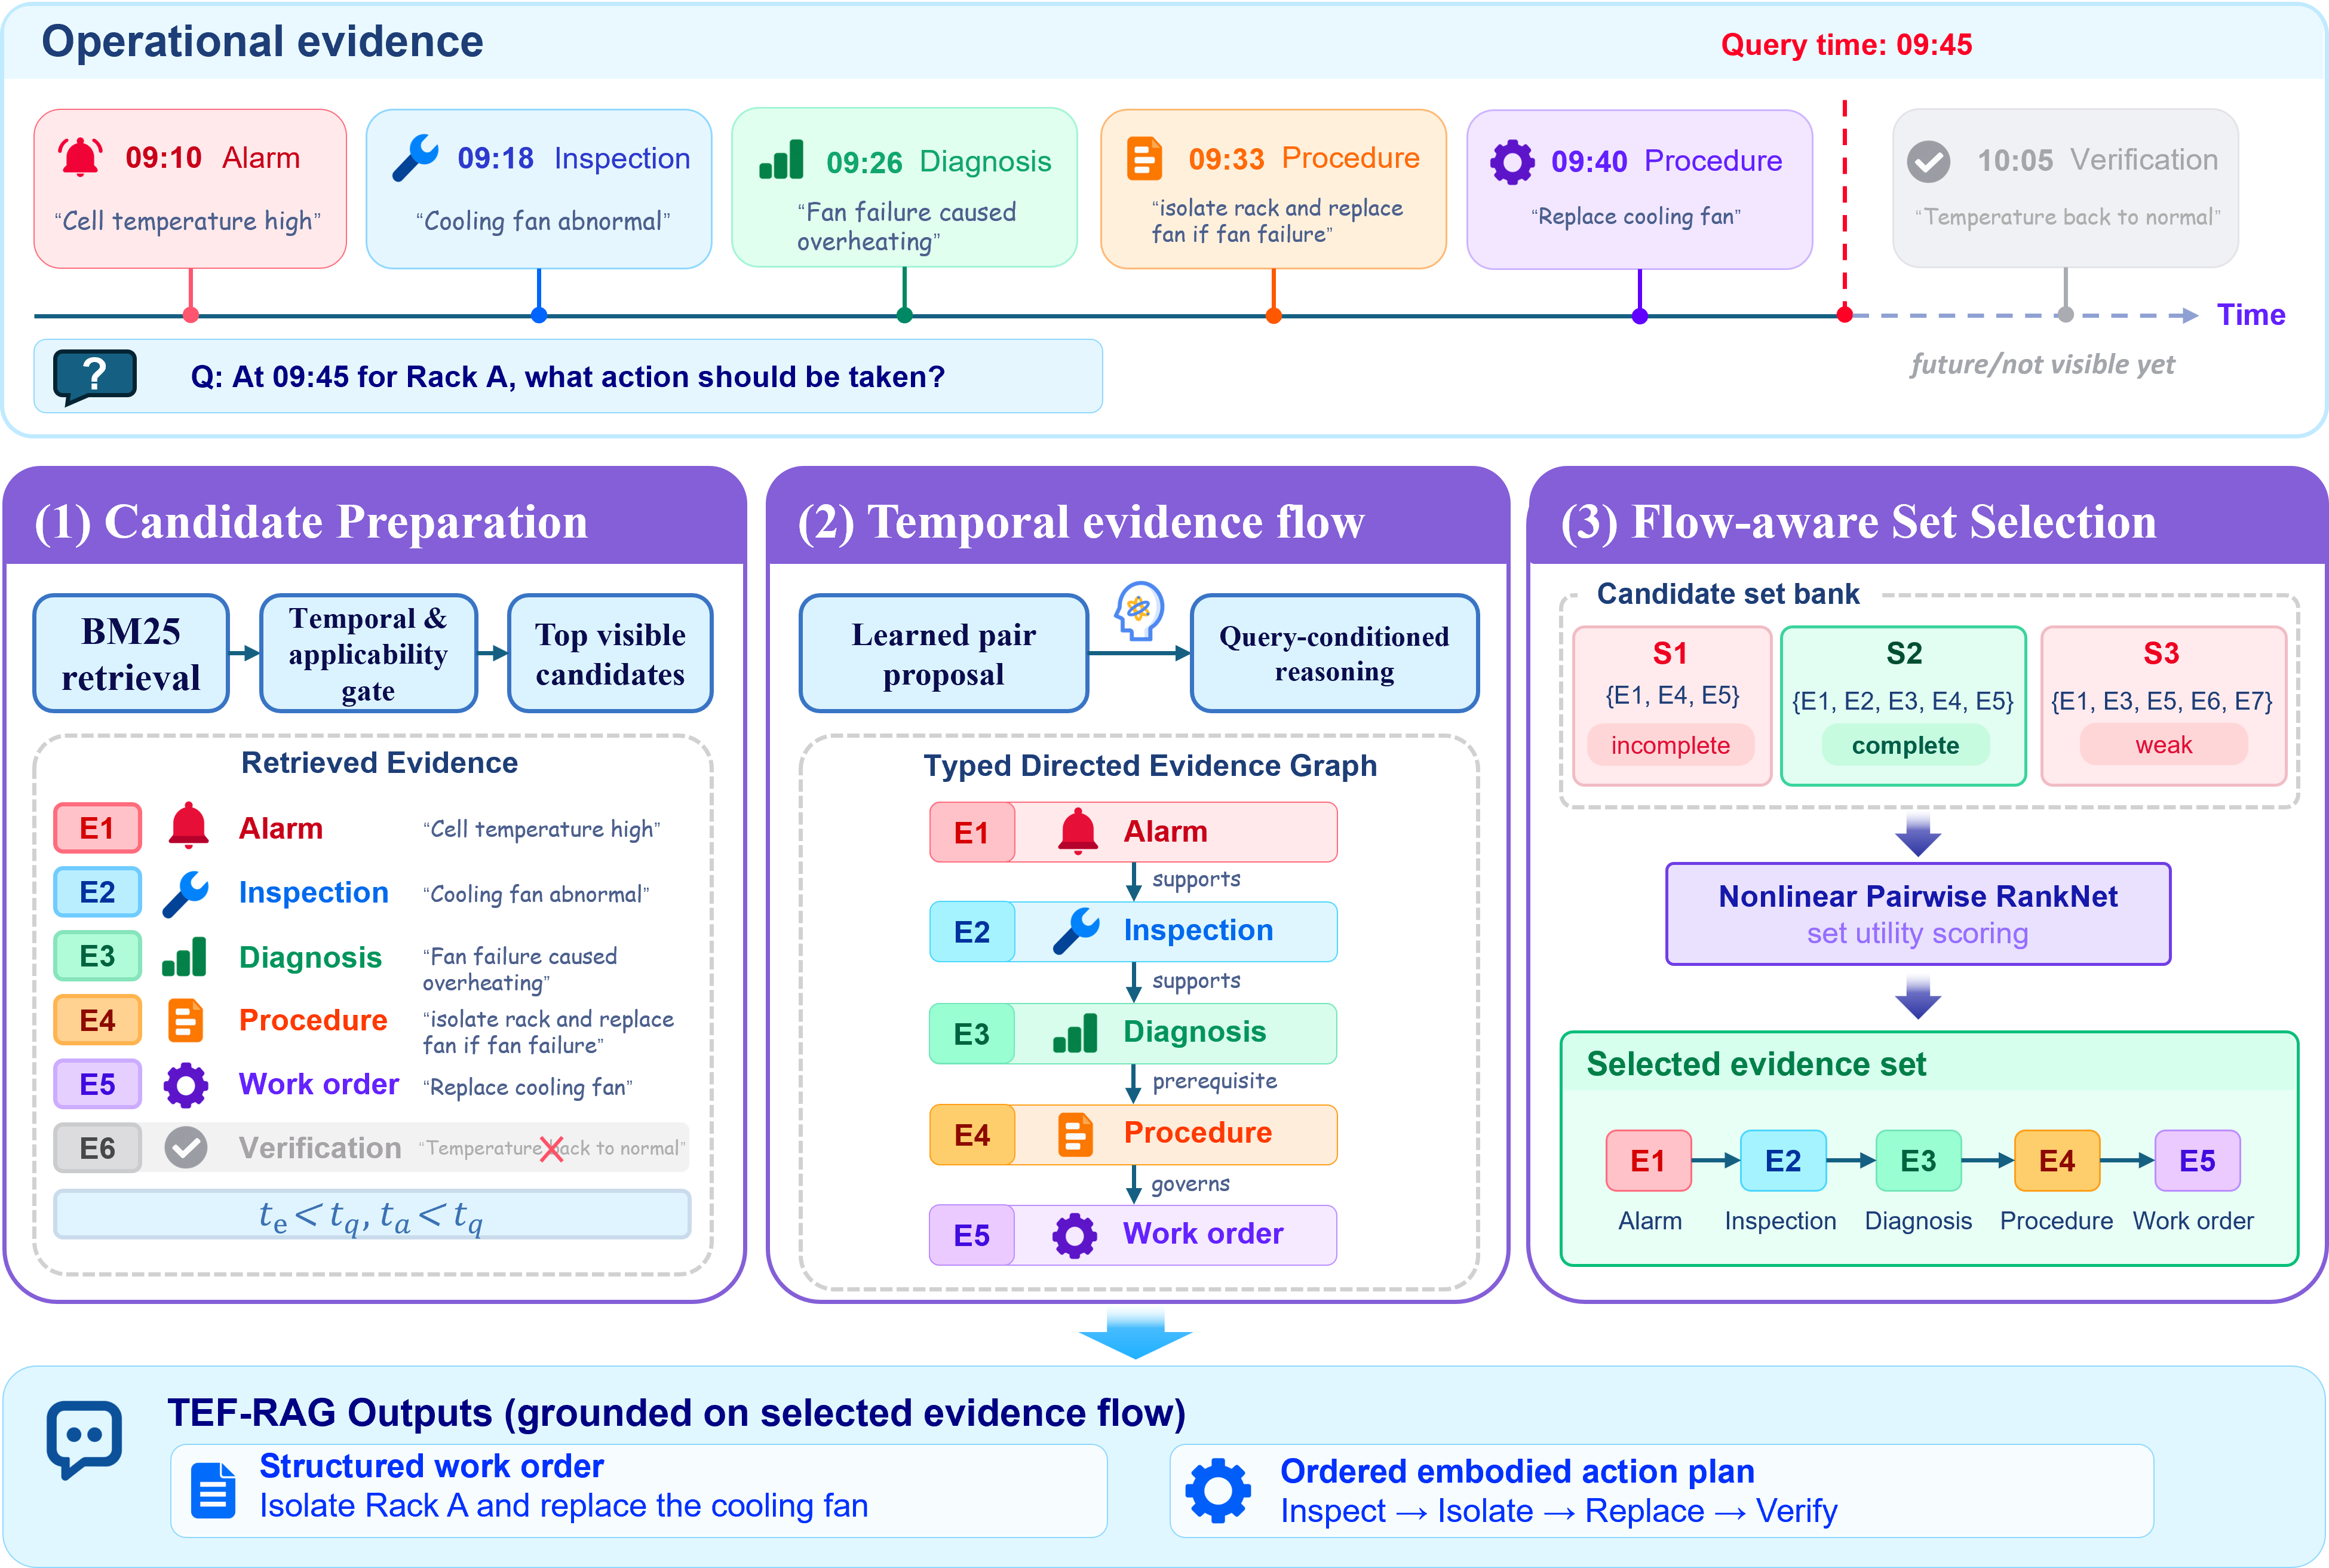
\includegraphics[width=0.96\textwidth]{figures/tef_rag_overview.png}
    \caption{TEF-RAG 总体框架。系统首先从查询时刻合法的记录中选择候选证据对，随后构建查询条件化的时序证据流。非线性成对排序器从候选集合空间中选择至多五条记录构成证据流，并将其作为受控上下文输入共享的下游生成器。}
    \label{fig:tef_overview}
\end{figure*}

\subsection{候选证据准备与时间合法性}

TEF-RAG 首先对异构原始记录进行统一的合法性检查。若记录对应错误资产、描述的是查询时刻之后发生的事件、直到查询时刻之后才对系统可用，或属于对当前型号或时间区间不适用的规程，则会被直接剔除。该阶段并不学习相关性，而是建立后续模型不可越过的知识边界。

在合法集合 $\Candidates_q$ 内，BM25 首先产生一个较宽的候选池。随后利用检索时可获得的特征形成 Top-30 搜索池，这些特征包括词法相关性、时间新近性以及与查询所需任务角色的兼容性。该候选池的目的在于尽可能保留召回，而不是直接决定最终输出。若合法候选少于五条，则系统保留较短的结果，不进行人为填充。

\subsection{学习式证据对提议}

若对搜索池中的所有有序证据对都进行语义关系推理，其计算成本将随候选数呈二次增长。因此，TEF-RAG 首先学习一个轻量级证据对提议器，对每个时间上合法的证据对 $(e_i,e_j)$ 估计其值得送入关系推理阶段的概率：
\begin{equation}
p_{ij}
=
\sigma\!\left(
\mathbf{w}^{\top}\phi_p(q,e_i,e_j)+b
\right).
\label{eq:pair_proposal}
\end{equation}

其中，$\phi_p(q,e_i,e_j)$ 表示查询 $q$ 与证据对 $(e_i,e_j)$ 的特征表示，包括查询与两条记录的文本相关性、两条记录之间的相似度、事件类型、时间间隔以及与版本替代相关的信息。如果某个证据对在训练数据中标注的参考证据流里实现了一个必需关系，则将其作为正样本；其余时间上合法的证据对作为负样本。随后使用逻辑回归学习候选证据对的优先级，仅将高分证据对送入后续关系推理模块。

在本文评估配置中，一个 Top-30 搜索池最多包含
$\binom{30}{2}=435$ 个按时间有序的候选证据对，
而证据对提议器仅保留得分最高的 32 对用于后续关系判断。
因此，当搜索池包含 30 条记录时，关系判断次数最多可减少约 92.6\%。
证据对提议的主要作用是控制计算预算：在保持确定性时间方向约束的前提下，仅将得分最高的候选证据对交给语义关系推理。

\subsection{查询条件化的时序证据流}

对于每个保留的候选证据对，TEF-RAG 使用查询条件化的 LLM 关系判断器。该判断器同时读取查询以及两条证据记录的文本和元数据，并输出
\begin{equation}
h_{\eta}(q,e_i,e_j)
\rightarrow
(r_{ij},c_{ij}),
\end{equation}
其中，$r_{ij}\in\Rels$，$c_{ij}\in[0,1]$ 为关系置信度。只有被预测为存在有效关系且置信度超过阈值的证据对才会加入图中；未被赋予有效关系或置信度低于阈值的证据对将被丢弃。关系判断器使用的固定提示词见附录~\ref{app:relation_prompt}。

候选证据记录被视为图节点，两条记录之间识别出的语义关系表示为有向边。对于查询 $q$，时序证据流图定义为
\begin{equation}
\FlowGraph_q=(V_q,E_q),
\end{equation}
其中，$V_q$ 为候选证据集合，$E_q$ 为证据关系集合。每条有向关系边可写为 $(e_i,r,e_j)$，表示证据 $e_i$ 通过关系 $r$ 指向证据 $e_j$，其中 $r\in\Rels$。

关系词表包含面向过程的关系，例如支持、约束、限定、对比、前置条件、保留不确定性、消解、替代、更新和验证。边的方向遵循事件时间，或显式的前置条件/更新方向，因此图结构可以出现分支与汇合，而不被强制限制为单一路径。

与静态知识图谱不同，$\FlowGraph_q$ 是查询条件化的：同一对记录在不同查询下可能承担不同任务角色。关系判断器也不能越过第~\ref{sec:problem} 节定义的合法性边界；因此，晚到证据、未来事件和不适用规程不能通过语义推理重新进入候选集合。

\subsection{候选证据集合构造}

关系图构建完成后，TEF-RAG 比较不同的证据组合，而不是继续独立排序单条记录。若直接枚举整个搜索池中的所有五记录组合，代价较高，因此我们将排序范围限制在由以下过程生成的候选集合内。

具体而言，我们从得分最高的证据节点中枚举五记录组合，以覆盖不同的高相关记录组合；同时保留前序检索步骤生成的集合，并围绕这些集合执行单记录替换，使那些排名较低但能够补齐必需任务角色的证据有机会进入候选集合库。

对于每个集合 $\Selected$，我们提取集合级表示 $\phi_s(q,\Selected,\FlowGraph_q)$。最终模型使用 62 个特征，涵盖：
\begin{itemize}
    \item 节点相关性、时间得分与角色兼容性的统计量；
    \item 事件类型与来源类型的覆盖情况；
    \item 有效内部边数量、边置信度、连通分量数量以及最长有向路径；
    \item 时间跨度、平均事件间隔以及来源/文本多样性；
    \item 对冗余、缺失角色和孤立节点的惩罚信号。
\end{itemize}
这些特征共同描述所选证据作为一个整体是否形成完整的任务支撑结构，而不只是重复单个节点的分数。

\subsection{非线性成对集合排序}

最终排序器采用非线性 RankNet~\cite{burges2005ranknet}。令
\begin{equation}
s_{\theta}(q,\Selected)
=
\operatorname{MLP}_{\theta}
\!\left(
\phi_s(q,\Selected,\FlowGraph_q)
\right).
\end{equation}
最终阶段对证据集合进行成对偏好学习。对于同一查询，候选集合通常同时包含多个完整和不完整的备选方案。我们构造训练对
$(\Selected_i^+,\Selected_j^-)$，
其中 $\Selected_i^+$ 是能够形成完整参考证据流的候选集合，$\Selected_j^-$ 则是缺失必需证据或具有不完整关系结构的候选集合。

对于每个训练对，排序器被训练为给完整集合更高的分数：
\begin{equation}
\ell(q,\Selected_i^+,\Selected_j^-)
=
-\log \sigma\left(
s_{\theta}(q,\Selected_i^+)
-
s_{\theta}(q,\Selected_j^-)
\right).
\label{eq:ranknet_pair_loss}
\end{equation}

最终目标是在所有训练对上取平均损失：
\begin{equation}
\mathcal{L}
=
\frac{1}{|\mathcal{P}|}
\sum_{(q,\Selected_i^+,\Selected_j^-)\in\mathcal{P}}
\ell(q,\Selected_i^+,\Selected_j^-),
\label{eq:ranknet_loss}
\end{equation}
其中，$\mathcal{P}$ 表示训练期间构造的全部候选集合对。

在第一轮训练中，负样本首先依据规则式集合评分进行优先选择。该评分综合单条证据质量、集合内部关系、任务角色覆盖、内容冗余以及孤立证据，其完整定义见附录~\ref{app:hand_score}。这些集合往往包含若干高度相关的记录，但仍缺失必需的证据类别或关系，因此比随机负样本更难区分。我们还保留少量组成上具有多样性的负集合，以提高训练样本的多样性。

第一轮训练完成后，使用当前排序器重新评分全部负集合，并将其中得分最高但失败的集合选作难负样本。尽管这些集合已知无法形成完整参考证据流，但当前模型最容易将它们排到靠前位置。第二轮训练使用这些难负样本进一步细化完整集合与不完整集合之间的判别边界。

\subsection{面向具身运维生成器的接口}

TEF-RAG 的输出不是低层机器人控制命令，而是供下游具身执行使用的证据上下文。共享的下游生成器接收查询与检索证据，生成标准化工单和具有依赖关系的动作计划；这些结构化输出随后可以传递给规划器、约束检查器或机器人执行模块。

为隔离检索质量本身的影响，所有对比方法共享同一个下游生成器。生成器只接收查询和当前检索方法选出的证据记录，不接收方法名称、检索分数或 TEF 图结构。固定的生成提示词见附录~\ref{app:generation_prompt}。本文的评估止于结构化工单与动作计划，不将闭环机器人执行或现场安全认证视为已经解决的问题。
